\documentclass[11pt]{article}
%Required: You must have these
\usepackage{graphicx}
\usepackage{tabularx}
\usepackage{natbib}
\usepackage{array}
\usepackage{amsmath}
%\usepackage[backend=bibtex]{biblatex}
\setkeys{Gin}{width=0.8\textwidth}
%\setlength{\captionmargin}{30pt}
\setlength{\abovecaptionskip}{10pt}
\setlength{\belowcaptionskip}{10pt}
 \topmargin -1.5cm 
 \oddsidemargin -0.04cm 
 \evensidemargin -0.04cm 
 \textwidth 16.59cm
 \textheight 23.94cm 
 \parskip 7.2pt 
\renewcommand{\baselinestretch}{1.2} 	
\parindent 0pt
\usepackage{lineo}
\linenumbers

\bibliographystyle{..//refs/styles/besjournals.bst}
\usepackage{xr-hyper}
%\usepackage{hyperref}
\externaldocument{SUPPperiodicity2021}

\title{Experimental designs for testing the interactive effects of temperature and light in ecology and the problem of periodicity }
\date{}
\author{D.M. Buonaiuto $^{1,2,a}$,M. Donahue$^{3}$, E.M. Wolkovich$^{4}$}

\begin{document}
\maketitle
\noindent \emph{Author affiliations:}\\
\noindent $^1$Arnold Arboretum of Harvard University, Boston, Massachusetts, USA. ORCID: 0000-0003-4022-2591\\
$^2$Department of Organismic and Evolutionary Biology, Harvard University, Cambridge, Massachusetts, USA \\
$^3$Hawai'i Institute of Marine Biology, University of Hawai'i at Manoa, Kan‘eohe, HI, USA.\\
$^4$Forest \& Conservation Sciences, Faculty of Forestry, University of British Columbia, Vancouver, British Columbia, Canada\\
$^a$Corresponding author: 617.823.0687; dbuonaiuto@g.harvard.edu\\
\pagebreak
\maketitle
\section*{Abstract}
\begin{enumerate}
\item Temperature and light cues interact to control many biological processes. Experiments in controlled environments give researchers the ability to manipulate these environmental cues independently, and can be designed to robustly quantify their individual and interactive effects on any particular biological activity. Testing the interactive effects of multiple environmental cues require experimental treatments to be fully independent, and any unmeasured experimental covariation among treatments can result in the misestimation of cues effects. 

\item  Using a database of controlled environment experiments on the spring phenology of woody plants as a case study, we highlight how a common experimental design to parse the interactive effects of temperature and photoperiod introduces latent experimental covariation of photo- and thermo-period. Using data simulations, algebraic corrections  and a comparative analysis of published experiments, we demonstrate how the unmeasured cue covariation in this commonly used experimental set-up biases statistical inference regarding the relative contribution of light and temperature cues to phenological variation.

\item We identify this experimental covariation in more than 40\% of published phenology studies that manipulate photoperiod. Our analyses demonstrate that this experimental covariation of thermo- and photo-periodicity results in the overestimation of the effect of photoperiod and the underestimatition of forcing effects and their interactions on phenology, which may, in part, explain why the significance of photoperiod cues for spring phenology is currently debated in the literature.

\item Accurate forecasting of how varying environmental conditions impacts the dynamics of biologcial events requires the accuate quantification of cues responses. To this end, we present several alternative experimental designs that can provide more robust estimations of the relative effects of temperature and photoperiod on phenology, and any other biological processes that is controlled by these temperature and light cues.
%283 words
\end{enumerate}

\textbf{Keywords:} phenology, photoperiod, thermoperiod, growth chamber, cues, light, temperature, full-factionial \\
2485 words, 4 figures
\section*{Introduction}
%Temperature and light dictate numerous biological processes including....\textit{list here}\citep{}. These cues often interact in complex ways, and a major goal of biology is to quantify their both individual and interactive effects on biological activity \citep{}. This effort has only become more critical in recent decades as such measurements are essential for accurately predicting organisms' response to anthropogenic global change and informing biodiversity conservation planning and practices \citep{}.\\
\noindent Across the tree of life, temperature and light availability shape a number of important biological processes including growth and metabolic rates \citep{MacLean:2019aa} sex determination \citep{Brown:2014vn}, acclimatization to seasonal environments \citep{Hamilton2016} and the timing of life cycle transitions (phenology) \citep{Forrest2010}. These biological responses in turn dictate broad scale ecological processes and patterns ranging from biogeochemical cycling \citep{Piao2007} to species range limits \citep{Chuine2001}. Characterizing the specific dynamics of how these environmental factors synergistically affect biological processes across a wide range of taxa has become even more important as anthropogenic global change continues to expose organisms to novel environmental conditions \citep{Portner:2008vd}.

%It is difficult to evaluate the individual effects of temperature and light cues and their interactions in \textit{in situ} observational studies because temperature and light variables tend to co-vary in nature \citep{}. However, well designed experiments in controlled environments (e.g. growth chambers, greenhouses, mesocosm) can be used to manipulate temperature and light variables independently, allowing for robust comparisons of their individual and interactive contributions to biological processes. Indeed, this approach has provided many fruitful insights regarding temperature and light signaling over the last century \citep{} and has great potentially to continue to advance fundamental and applied biological inquiries in the decades to come \citep{}.\\
\noindent Because temperature and light availability often co-vary in the field (for example, in most temperate ecosystems, daylength and temperature both increase as the season progresses \citep{Rosenberg1974}) it can be difficult to disentangle their relative contributions to biological processes. In contrast, experimental manipulations of climate variables in artificial environments can mechanistically characterize biological responses to environmental fluctuations \citep{Ettinger:2020aa,Primack2015}. Growth chambers of all shapes and sizes have been used to this end \citep{Downs:1980us} and these efforts have greatly advanced researchers' understanding of the fundamental biology of a wide variety of organisms and their ability to predict the responses to current and future climate change \citep{Stewart:2013wz}.

However, controlled environment experiments have their own challenges. Experimentalists must balance biological realism with statistical inference, experimental effort with statistical power, and account for the effects of unmanipulated or unmeasured variables \citep{schneiner2001}. Because biological responses to the environment are generally the product of complex interactions between multiple environmental signals \citep{Casal:2002vz}, seemingly small choices about experimental design can generate significant differences in outcomes. Experimental treatments are rarely standardized among researchers even within disciplines \citep{limitingcues} and these complexities may in part contribute to many discrepancies between experimental studies and observation data \citep{Poorter:2016aa}. Even with these limitations, growth chamber studies remain a powerful tool for mechanistically assessing organismic responses to the environment provided that the implications of treatment designs are well understood and well matched with the scope of the research question. 

As technology advances and experiments become more complex, researchers can manipulate more variables and multiple axes of variation (e.g. temperature, amplitude, periodicity, wavelength) at the same time. Yet these efforts may tradeoff between biological realism and statistical inference. Through investigating the literature of experiments with plant phenology (timing of recurring life cycle events, e.g. leaf budburst, flowering), we found that experiments that manipulate both photo- and thermo- periodicity often introduce a latent covariation between light and temperature experimental treatments that may misrepresent the effects of each of these environmental variables, and the interaction between them. Below, we begin by briefly detailing how temperature and light treatments are generally applied in experimental phenology studies and review the minimum experimental elements required to robustly test interactions between two or more environmental variables. We then detail the problem of inference that can arise manipulating the periodicity of both temperature and light in experiments and demonstrate the extent to which this is an issue with mathematical and experimental examples. Finally, we conclude by outlining several possible solutions for overcoming these issues.  While, our example deals with phenology of temperate woody plants, the issues and solutions we present below are broadly applicable to studies of any other organisms and biological processes that utilize temperature and daylength signals. 

\section*{Estimating phenological cues from experiments}
Decades of experimental work in growth chambers have demonstrated that temperature (both cool temperatures in fall/winter and warming temperatures in spring) and photoperiod are the primary cues of phenology for plants in the temperate/boreal zones \citep{Ettinger:2020aa}. While exposure to cool winter temperatures (chilling) strongly impacts phenology \citep{Laube2014}, we focus here on warm temperature treatments and light treatments, because controlled chilling treatments with light are uncommon (\citep{limitingcues}). Choices that about how to apply these two treatments in particular that can compromise inference on their effects, so we will focus of these two cues.

While a large variety of experimental designs have been used to study plant phenology, generally phenology experiments tend to manipulate two major axes of light and warm temperature variation:
\begin{enumerate}
\item \underline{Intensity:} The amount or quality of a variable. Here we define temperature intensity as the amount of heat present in the system (measured in degrees). In the phenology literature this measurement is generally referred to as forcing. We define light intensity as the luminosity or irradiance present in the system (measured in lumens or watts). 
\item \underline{Periodicity:} The interval at which the intensity of the variable is applied. Hereafter, we refer to the periodicity of light as photoperiod (often used synonomously with ``daylength") and the periodicity of temperature as thermoperiod. 
\end{enumerate}
For phenology, photoperiodicity is generally considered the primary light cue for plants (\citep{WAY:2015aa}, though see \citep{Brelsford2018,Cober1996} regarding light intensity and phenology). For temperature, conventionally both intensity and periodicity drive phenological activity and several metrics (e.g. growing degree hours, thermal sums, growing degree days)  that combine these two axes have been developed \citep{Gu:2016wa}. The importance of thermo-intensity and periodicity is well supported; under natural conditions diurnal temperature fluctuations in temperate regions can be quite large in the spring, and studies have found that diurnal temperature variation strongly influences plant phenology \citep{Burghardt:2016uy}. In fact, even if thermoperiodicity is not an explicit treatment variable (i.e. manipulated systematically), incorporating it in experiments is essential for translating experimental results into real world predictions \citep{plants9101312}.

Like many other biological processes, recent advances have demonstrated that plant phenological responses are nonlinear, due largely to interactions between cues \citep{limitingcues,fu2015}, highlighting the need for experiments designed to evaluate the strength of these interactions. To have the statistical power to partition the individual and interactive effects of two or more variables, an experiment must:
\begin{enumerate}
\item Have at minimum of two treatment levels of at least two variables.
\item Treatment levels must be full factorial (Fig. \ref{fig:examp}a.). Full factorial designs are both balanced (Fig. \ref{fig:examp}b.)  and orthogonal (Fig. \ref{fig:examp}c.); which is to say that all possible treatment combinations are applied and each treatment is independent of all others \citep{cheng2016}.
\end{enumerate}

These two critical elements may seem obvious but can be conspicuously absent from many published studies. In the case of woody plant phenology, using a recently published database (OSPREE: Observed spring phenological responses in experimental environments \citep{wolkovich2019}) we found that out of 152 controlled environment experiments (across 93 studies) only 18 manipulated both light and forcing cues with a design that was both balanced and orthogonal. This notable dearth of robust tests of light and temperature interactions may stem from the common limitations of time, space, and resources that experimentalists often face, but it may equally relate to a fundamental issues that arises from the fact that these variables themselves are comprised of multiple axes of variably.\\
%\section{Axes of environmental variation in experiments and their implications}

\subsection*{The problem of periodicity}
A common approach in phenology experiments that seems to balance prior knowledge about the underlying physiology of phenology, biological realism and experimental inference is to vary photoperiodicity, and thermal intensity and periodicity \citep[e.g.][]{Flynn2018,Sanz-Perez:2009aa,Basler:2014aa}. For example, a basic experiment might include a long (12 hours) and short (8 hours) photoperiod treatment and a high (30/20$^{\circ}$C day/night) and low (20/10$^{\circ}$C day/night) temperature treatment. Note that in this case, the thermoperiodicity is not an explicit treatment (both high and low temperature treatments employ a diurnal fluctuation of 10 $^{\circ}$C), and is simply incorporated in the design to enhance biological realism. At first glance, this design appears to meet the criteria of a full factorial design, multiple treatment levels that are balanced and orthogonal, with high/low temperature treatments (mean 25$^{\circ}$ and 15$^{\circ}$C respectively) and long/short photoperiod treatments applied in all possible combinations.

Yet the orthogonality of this design is based on the assumption to a 12 hour thermoperiod. If, rather the thermoperiod is coupled with the photoperiod, this is not the case because the daily mean temperature of the long/high treatment will be higher than that of the short/high treatment, and the long/low treatment slightly warmer than the short/low.  %(Fig \ref{fig:ortho}a). %could also phase this in growing gregrees
This is because the warmer day time temperatures are applied for different duration across the high temperature treatments and clearly illustrated whe temperature is coverted to thermals sums. For example,  given a base temperature of 0$^{\circ}$C, a low forcing treatment of 20/10$^{\circ}$C day/night accrues 360 thermal units per 24 hours at when crossed with the long, 12 hours of photoperiod treatment while, and only 320 thermal units when crossed with the at 8 hour short photoperiod treatment.While this covariation among the photoperiod and temperature treatments is biologically realistic, it makes it statistically impossible to differentiate their independent and interactive effects on any given biological process.\\

This problem of inference that arises from the experimental covariation of thermo- and photoperiodicty is not limited only to studies seeking to directly compare the effects of photoperiod and forcing; it applies in any study evaluating the influence of photoperiod on biological activity, even if it is the only manipulated cue. Experimentally isolating the effect of photoperiod assumes that all other environmental variables are held constant. Similar to the case described above,% for comparing the interactive effects of photoperiod and forcing, 
the covariation of photoperiod and thermoperiod in an experiment where forcing was supposed to be a consistant ambient condition, would yeild a situation in which longer photoperiod treatments were also receiving more, unmeasured heating that the shorter photoperiod treatments. In this case, some amount of the perceieved photoperiod effect is due to the latent, increased forcing, and the true effect of photoperiod cannot be ascertained.

Of the 51 experiments in the OSPREE database that manipulated photoperid experimental, up to 43\% of them appear to include a covariation with theromoperiod. Of the 18 studies that manipulated both photoperiod and temperature interactively, we found that up to 55\% of them may have this issue, suggesting that the true interactive effects of these cues on spring phenology is still quite poorly characterized. This may be in part why the relative contribution of temperature and photoperiod cues to spring phenology remains a contentious debate in the phenology literature \citep{koerner2010a}.

\subsection*{Periodicity and inference}
If the lack of orthognonality introduced to experiments when photoperiod and thermoperiod covary is overlooked, regression models will overestimate the photoperiod effect and underestimate the forcing effect on spring phenology 
(Fig. \ref{fig:3d}a,b.). If experiments are designed to quantify the interaction between photoperiod and forcing, here too, the interactive effect will be underestimated due when compared to the true effect (Fig. \ref{fig:3d}c,d.). This is, in part because forcing is the variable with latent variation, and because studies repeatedly suggest that forcing is a more dominant cue than photoperiod for spring phenology \citep{CHUINE:2010wg,Zohner:2016uz,Gauzere2019}.%, therefore we should \emph{a priori} expect the covariation between photo- and thermo-period may result in an over-estimation of the photoperiod effect. %and a weaker estimate of the interaction between photoperiod and forcing. DB I checked this and we still underestimate photoperiod even when it is a stronger effect

\textbf{We can mathematically solve for how much of an estimated photoperiod effect is due to forcing---in experiments where they covary---by making several major asssumptions. If we assume forcing and photoperiod effects are additive, linear and there is no interaction between the two effects, then we can solve (algebraically) for the estimated effect of forcing and photoperiod given an orthogonal treatment design (see Fig. \ref{fig:3d}, Supporting info). Using estimates from one experiment that covaried forcing and photoperiod effects \citet{Flynn2018}, we found roughly two-thirds of the estimated photoperiod cue could be due to forcing effects.} % Lizzie says -- estimated effect of 4.5 in the paper, while in the supp we show 3 could be due to co-variation. 

While we are aware of no experiments that explicitly compare the effects of co-varying vs. independent photo- and thermo- periods, two phenology experiments in our lab utilized many overlapping treatment levels and species from the same sampling sites however in one study, \citet{Flynn2018}, photo- and thermo- period co-vary, while in the other \citet{Buonaiuto:2021ug}  photo- and thermo- period were varied independently. Comparing the cue estimates from these two studies offers an opportunity to test the theoretical and mathematical predictions, and further understanding the uncertainly in cue estimate due to periodicity.

We subset each dataset to include only the species shared among the two studies, and re-analyzed the data using Bayesian hierarchical models to compare difference in the photoperiod and forcing estimates (see Supplement for Methods). We found that the estimated differences in the mean response to photoperiod and forcing% and their interactions
among study designs were on the same order as our mathematical predictions, and that the un-coupled design estimated a weaker (less negative) photoperiod effect, and stronger forcing % and interaction
effect than the coupled experimental design (\ref{fig:compy},\ref{tab:esty}). \\

There are almost certainly other factors driving the differences between these experiments. Both were conducted in different years, sampled different individuals from the population, and used different methods for applying chilling pre-treatments \citep{Flynn2018,Buonaiuto:2021ug}. However, because this comparison is well matched to our mathematical predictions and prior knowledge about how temperature and photoperiod are expected to interacting in phenology, we argue that the influence of periodicity covariation on statistical inference is apparent enough to take seriously.\\

\section*{Paths Forward}
Above we have systematically demonstrated that experiments that co-vary thermoperiod and photoperiod cannot robustly differentiate the individual effect of temperature and photoperiod on a spring phenology (or any other biological process) or accurately quantify their interactive influence. Given the paucity of interactive studies in the literature, it is clear that more well designed studies will be needed to better characterize the effects of these cues. Below we offer several generalized experiment designs that improve statistical orthogonality of controlled environment experiments which could be further developed and adjusted to fit the needs of experimentalists across many sub-fields of biology.
\begin{enumerate}
\item \textbf{Covarying photo- thermo- period with quantified uncertainty}. It may be that the experimental design that best balances environmental realism, statistical inferences and translatability to observational studies are designs that co-vary periodicity to mimic natural systems (\ref{fig:ortho}a.). Moving forward, researchers using this design need to be aware of the non-orthogonality of this design, and be sure to present the uncertainty surrounding their cue effect estimates, which could be done using a similar mathematical approach to the one we present in this paper (see Supplement).

\item \textbf{Manipulate photoperiod and temperature intesity with no thermoperiodicity}. This approach allows for the maintenance of statistical orthogonality across treatment combinations (\ref{fig:ortho}b.). The main drawback is that this design sacrifices the biological realism of diurnal temperature variation, which may make it more difficult to translate estimates from experiments to real world applications.

\item \textbf{Compensitory diurnal temperature fluctions}. There are almost unlimited pairs of integers that can reduce to the same mean (e.g. $(24+26)/2 = (30+20)/2 = 25$) and the non-orthogonality of the mean daily temperature that arises in a coupled photo-thermoperiod design could be corrected for by proportionately increasing the diurnal temperature fluctuation of the short photoperiod treatment relative to the long treatments (\ref{fig:ortho}c.). However, if the differences between day and night temperature has a meaningful biological effect, this introduces another confounding, non-orthogonal factor for interpreting temperature and photoperiod effects. For example, the influence of day time warming of phenology can be as much as three times stronger than proportionate night time warming \citep{Rossi2017,Meng:2020ui}.

\item \textbf{Uncouple thermoperiod and photoperiod.} By varying thermoperiod and photoperiod independently (\ref{fig:ortho}d.), statistical orthogonality can be maintained across treatment. However, this approach may also introduce new artifacts that occur from the biological rather than statistical interactions between light and temperature \citep{Chew:2012wj}. For example, there is evidence that increasing temperatures in the first two hours of daylight can be almost as effective for stimulating shoot elongation as similar temperature increases for the whole photoperiod \citep{Erwin1998}. With this design, treatments must inherently differ in the amount of time the warmer daytime temperature extends into the dark nighttime light regime, introducing a new axes of non-orthogonality.
\end{enumerate}

In correcting one problem, each of these designs introduces another, which may in fact be an intrinsic property of any experimental manipulation. It would certainly be useful for researchers to explicitly test how cue estimates vary among these experimental designs, and which design is most useful for predicting phenology in the field under current and future climate conditions. In the meantime, we hope this treatment of the issue reminds experimentalists that we must continue to be thoughtful about matching design to the goals of a study, and being transparent about uncertainty around our experimental inference.

\section*{Author contributions}
DMB, MD and EMW conceived of the manscript; MD and EMW developed the algebraic solution; DMB performed the comparative analysis of the published studies; DMB led the writing of the manuscript. All authors contributed to writing and gave final approval for the submission.

\section*{Data Availability}
Data from the \cite{Flynn2018} study is available at the Harvard Forest Data Archevie (https://harvardforest1.fas.harvard.edu/exist/apps/datasets/showData.html?id=HF314) and from the \citet{Buonaiuto:2021ug} study available at Knowledge Network for Biocomplexity (https://knb.ecoinformatics.org/view/doi:10.5063/PG1Q4B). The R code used to analyse the data is available on github.

\bibliography{..///refs/periodicity.bib}

\begin{figure}[h!]
    \centering
 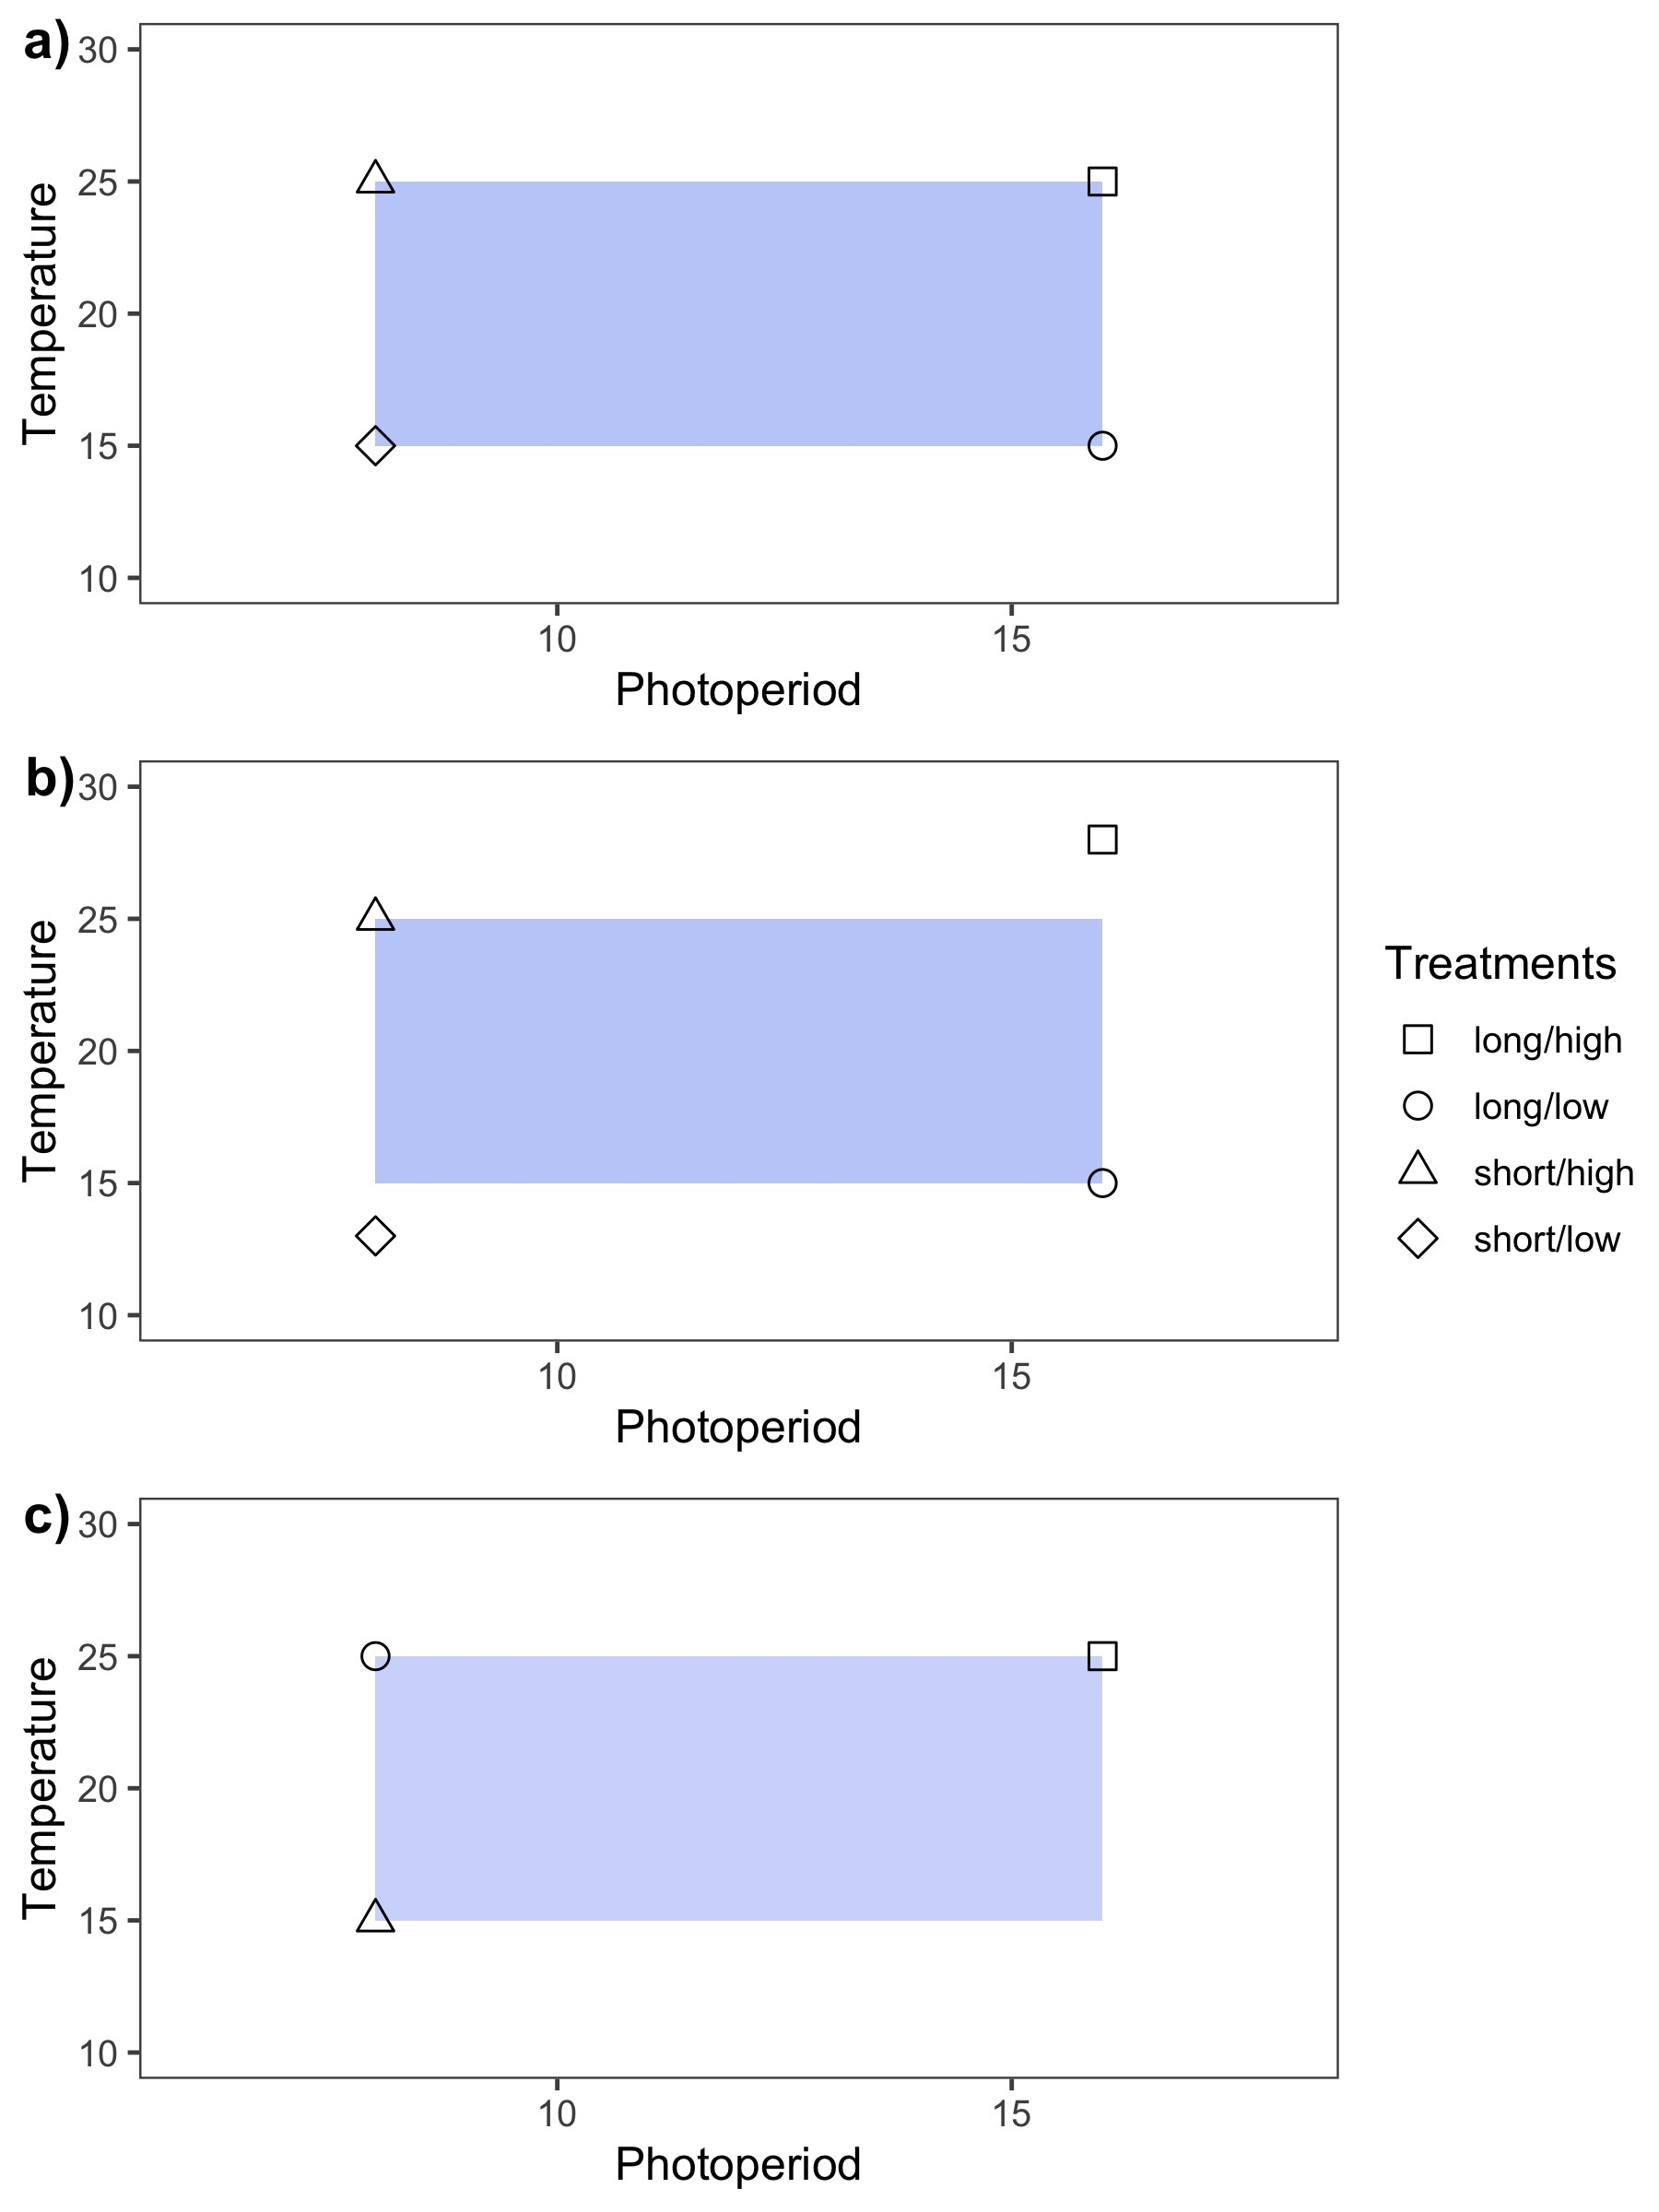
\includegraphics[width=.8\textwidth]{..//Plots/periodicity_figures/factorial.jpeg}
    \caption{Idealized experimental designs demonstrate three approaches for varying temperature and light treatment level in controlled environment experiments. Design \textbf{a)} is fully factorial in that treatments levels are balanced and orthogonal. This design is appropriate for testing interactions between two or more variables. In \textbf{b)} the design is balanced but not orthogonal. Non-orthogonality in experiments can arise when experimental covariation among the test variables is not accounted for. In \textbf{c)}, the experimental design is orthogonal but unbalanced. Lack of balance in experiments often arises due to time, space or resource limitations. }
    \label{fig:examp}
\end{figure}


 
 \begin{figure}[h!]
    \centering
 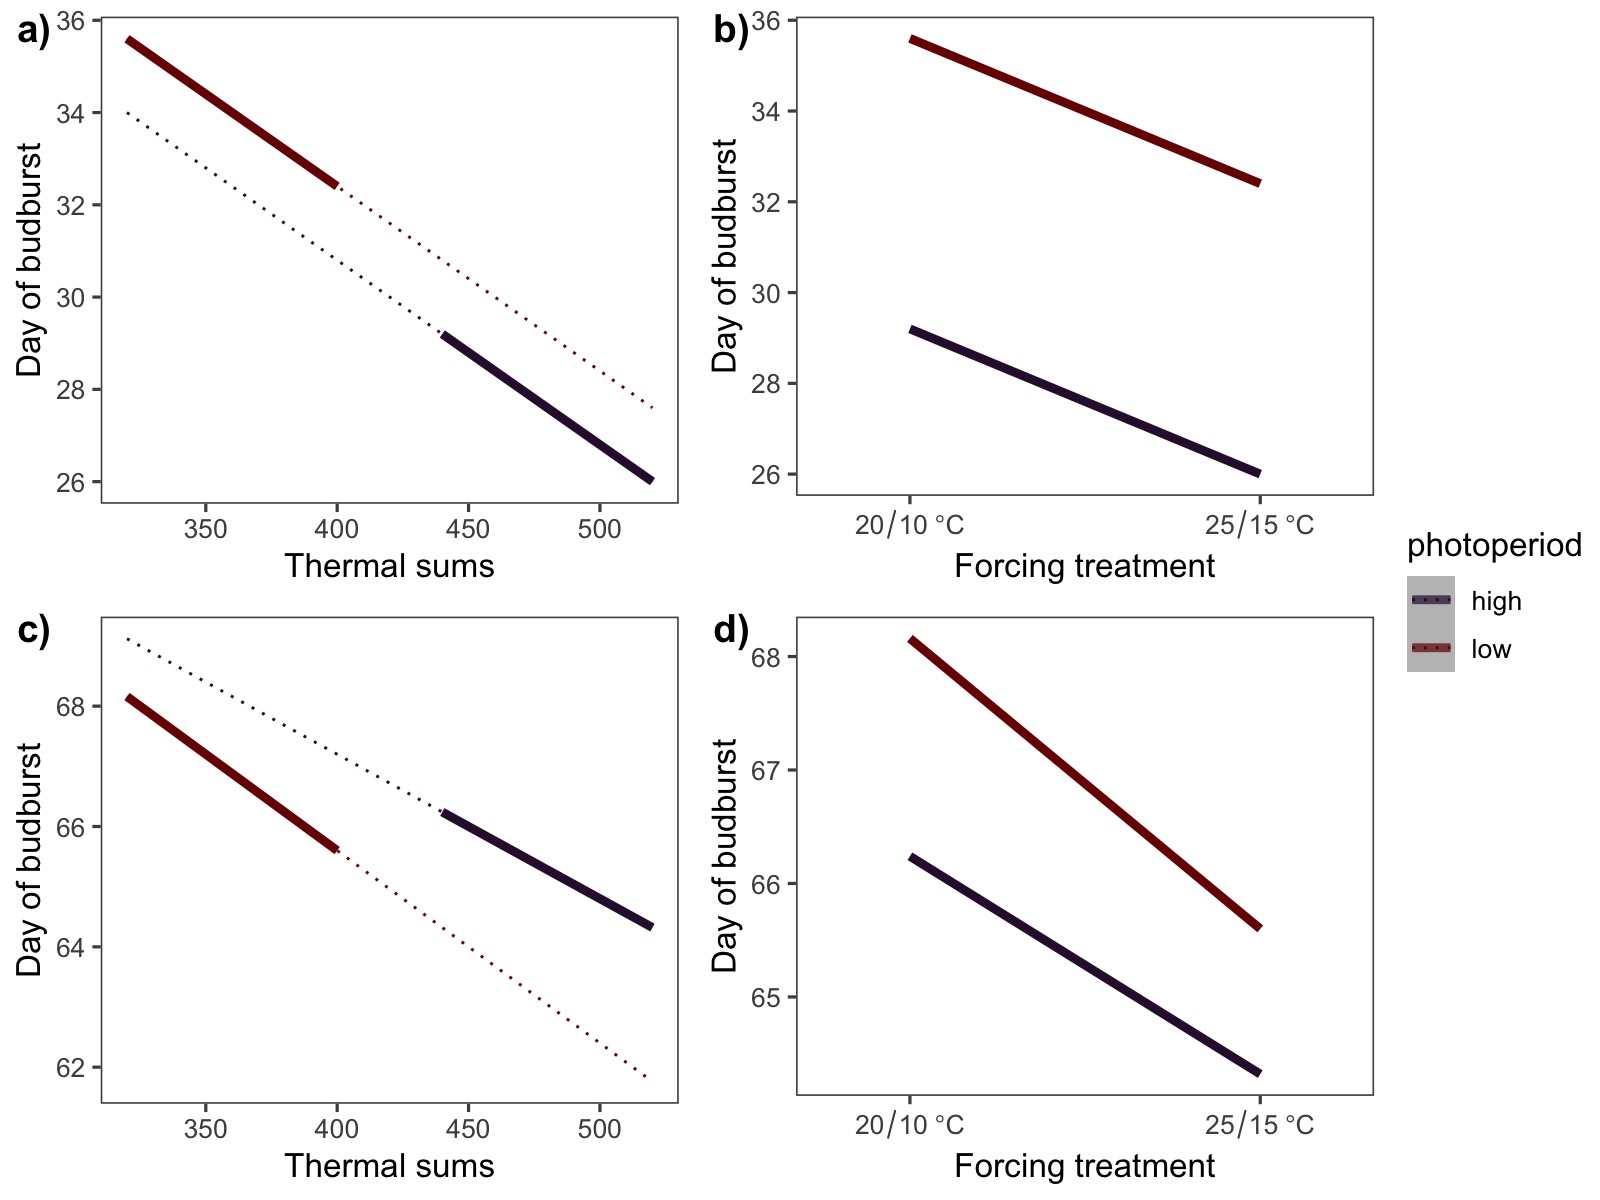
\includegraphics[width=.8\textwidth]{..//Plots/periodicity_figures/apparent.jpeg}
    \caption{Estimated effects of photoperiod and forcing on phenology. a) True effects no interactions. b) estimated effects . c) True effects with interactions. d) estmated effects.}
    \label{fig:3d}
\end{figure}
 
\begin{figure}[h!]
    \centering
 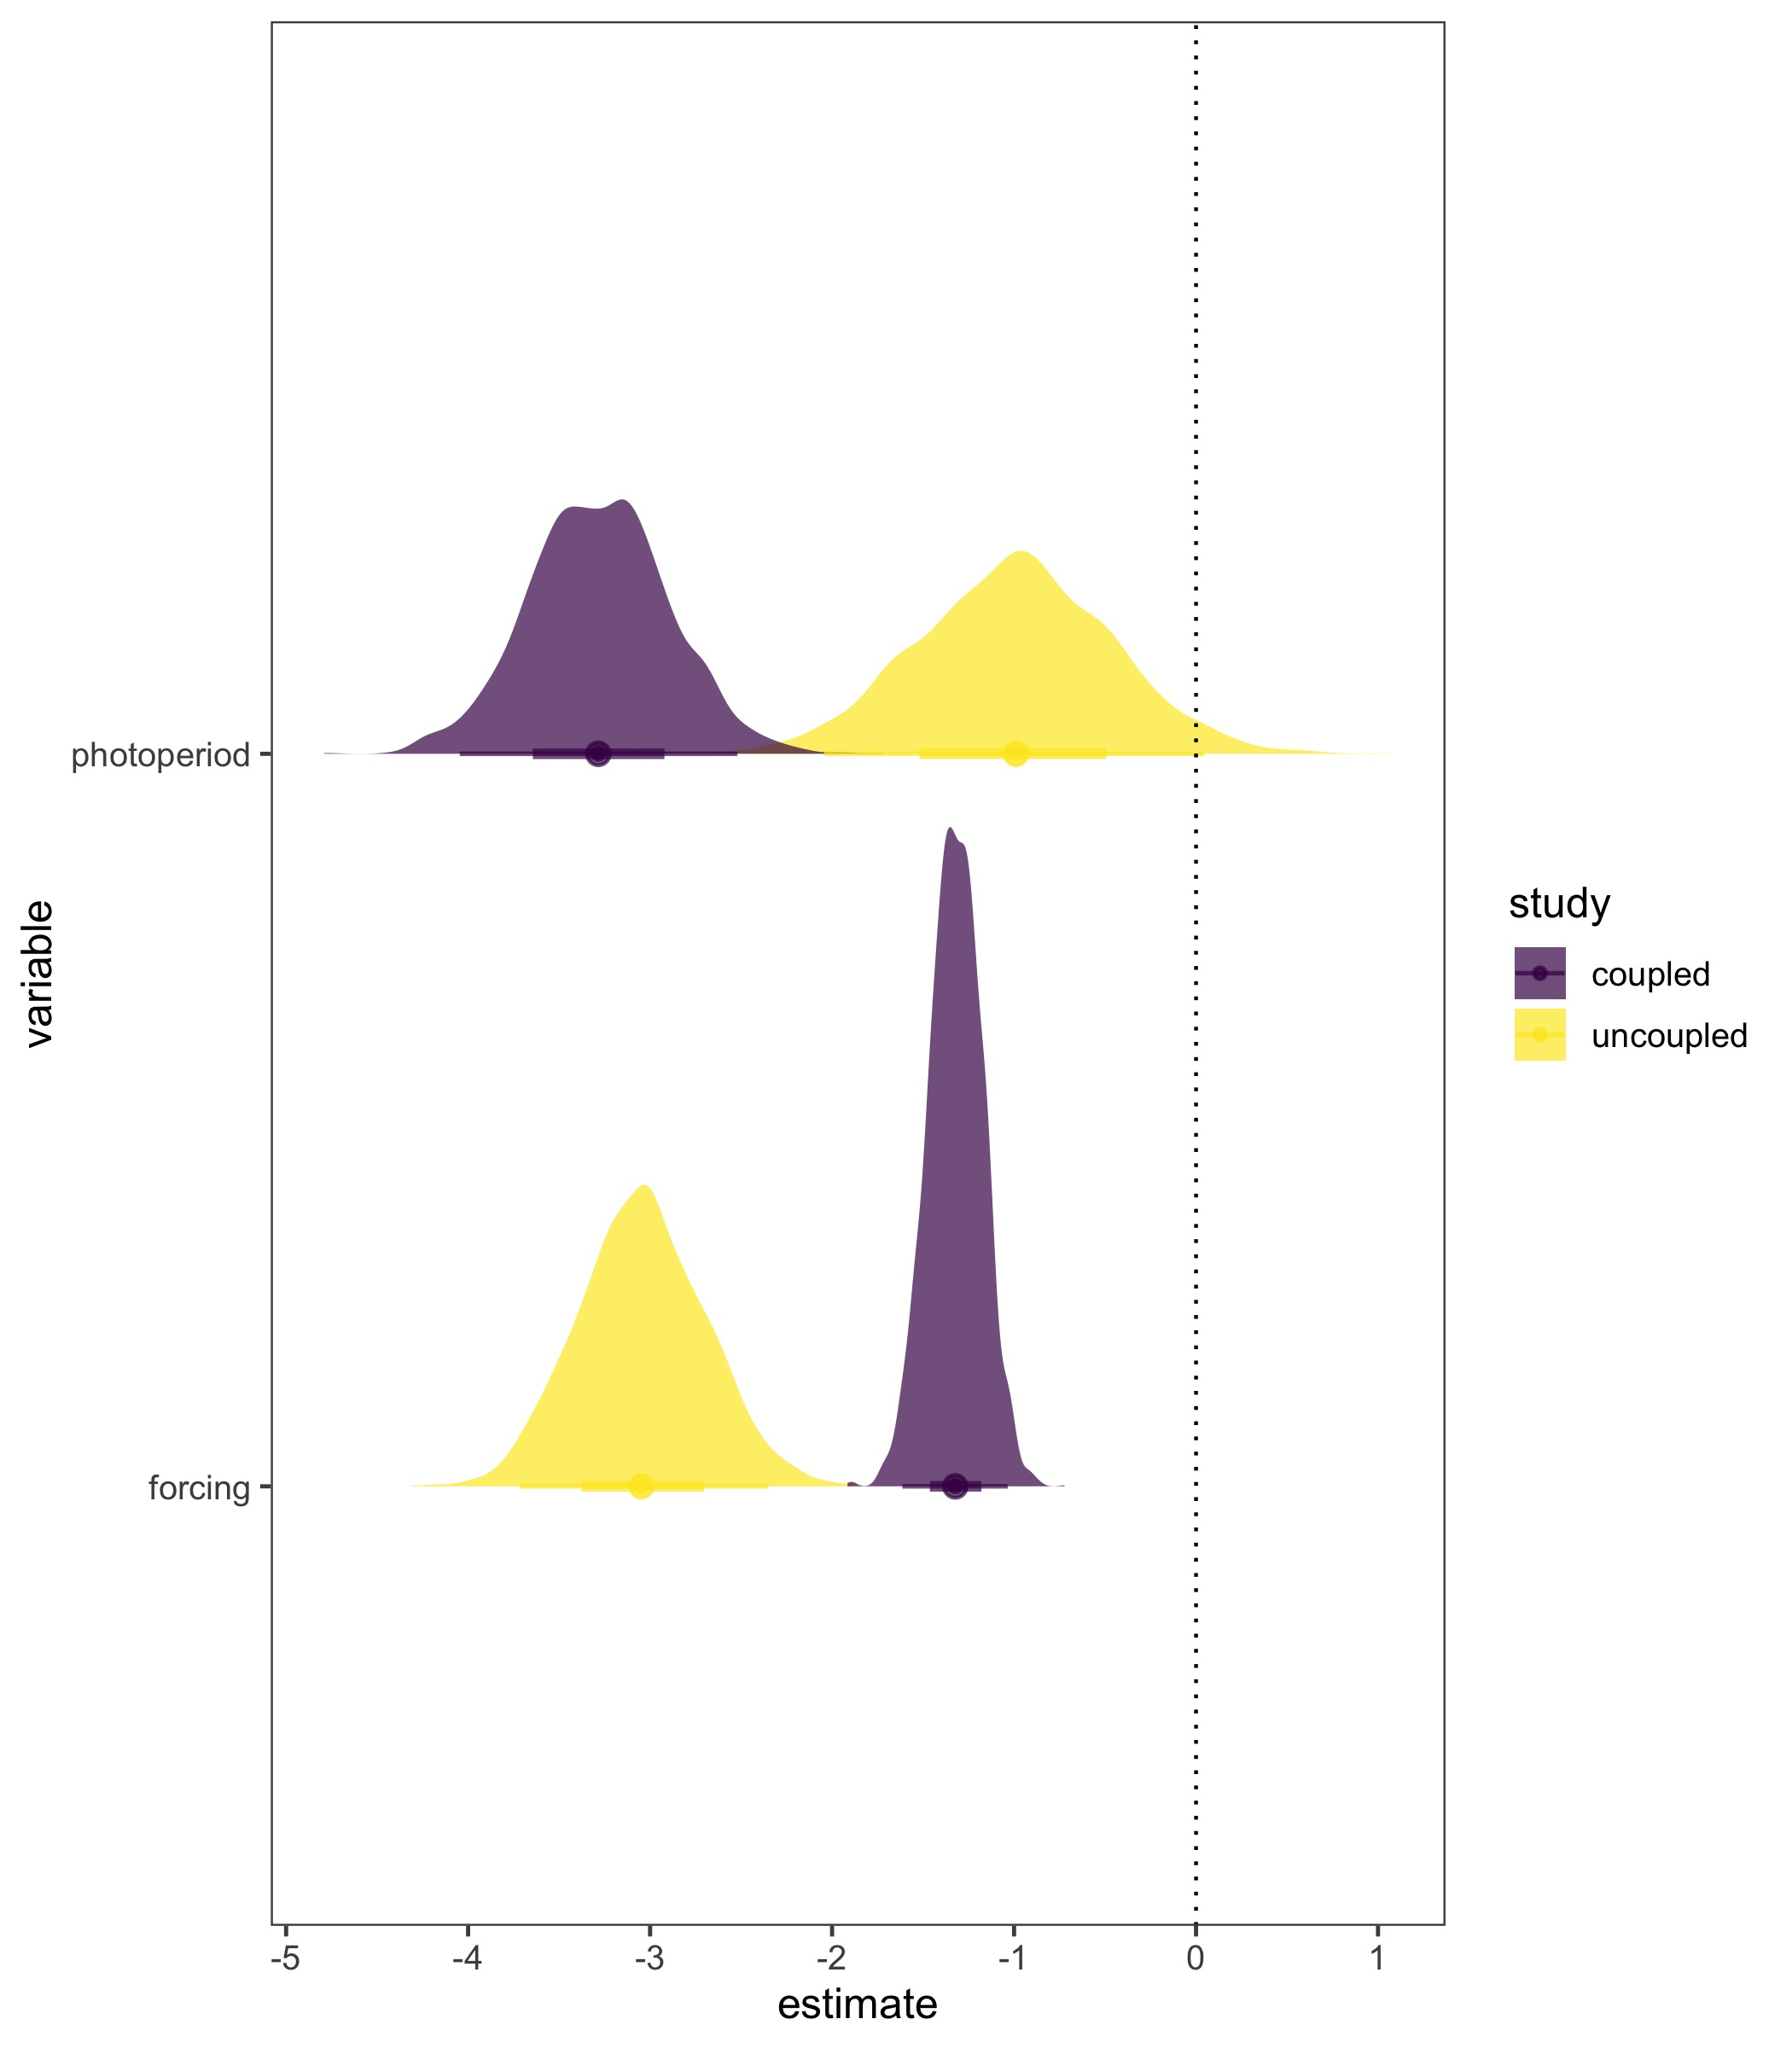
\includegraphics[width=\textwidth]{..//Plots/periodicity_figures/modelcomps.jpeg}
    \caption{Estimated effects of one hour increase in photoperiod and one degree C increase in forcing on the day of leaf expansion using an alternative methods of varying thermo-period relative to photoperiod. Dots indicate the estimated mean effect, thick and thin bars the 50\%  and 97.5\% credible intervals respectively. The full posterior distributions are also depicted for each parameter estimate. The colors represent the study design effect, with purple representing study design in which photo- and thermo-period co-vary, and yellow representing a design where there periodicity of each variable is independent of the other.} 
    \label{fig:compy}
\end{figure}

\begin{figure}[h!]
    \centering
 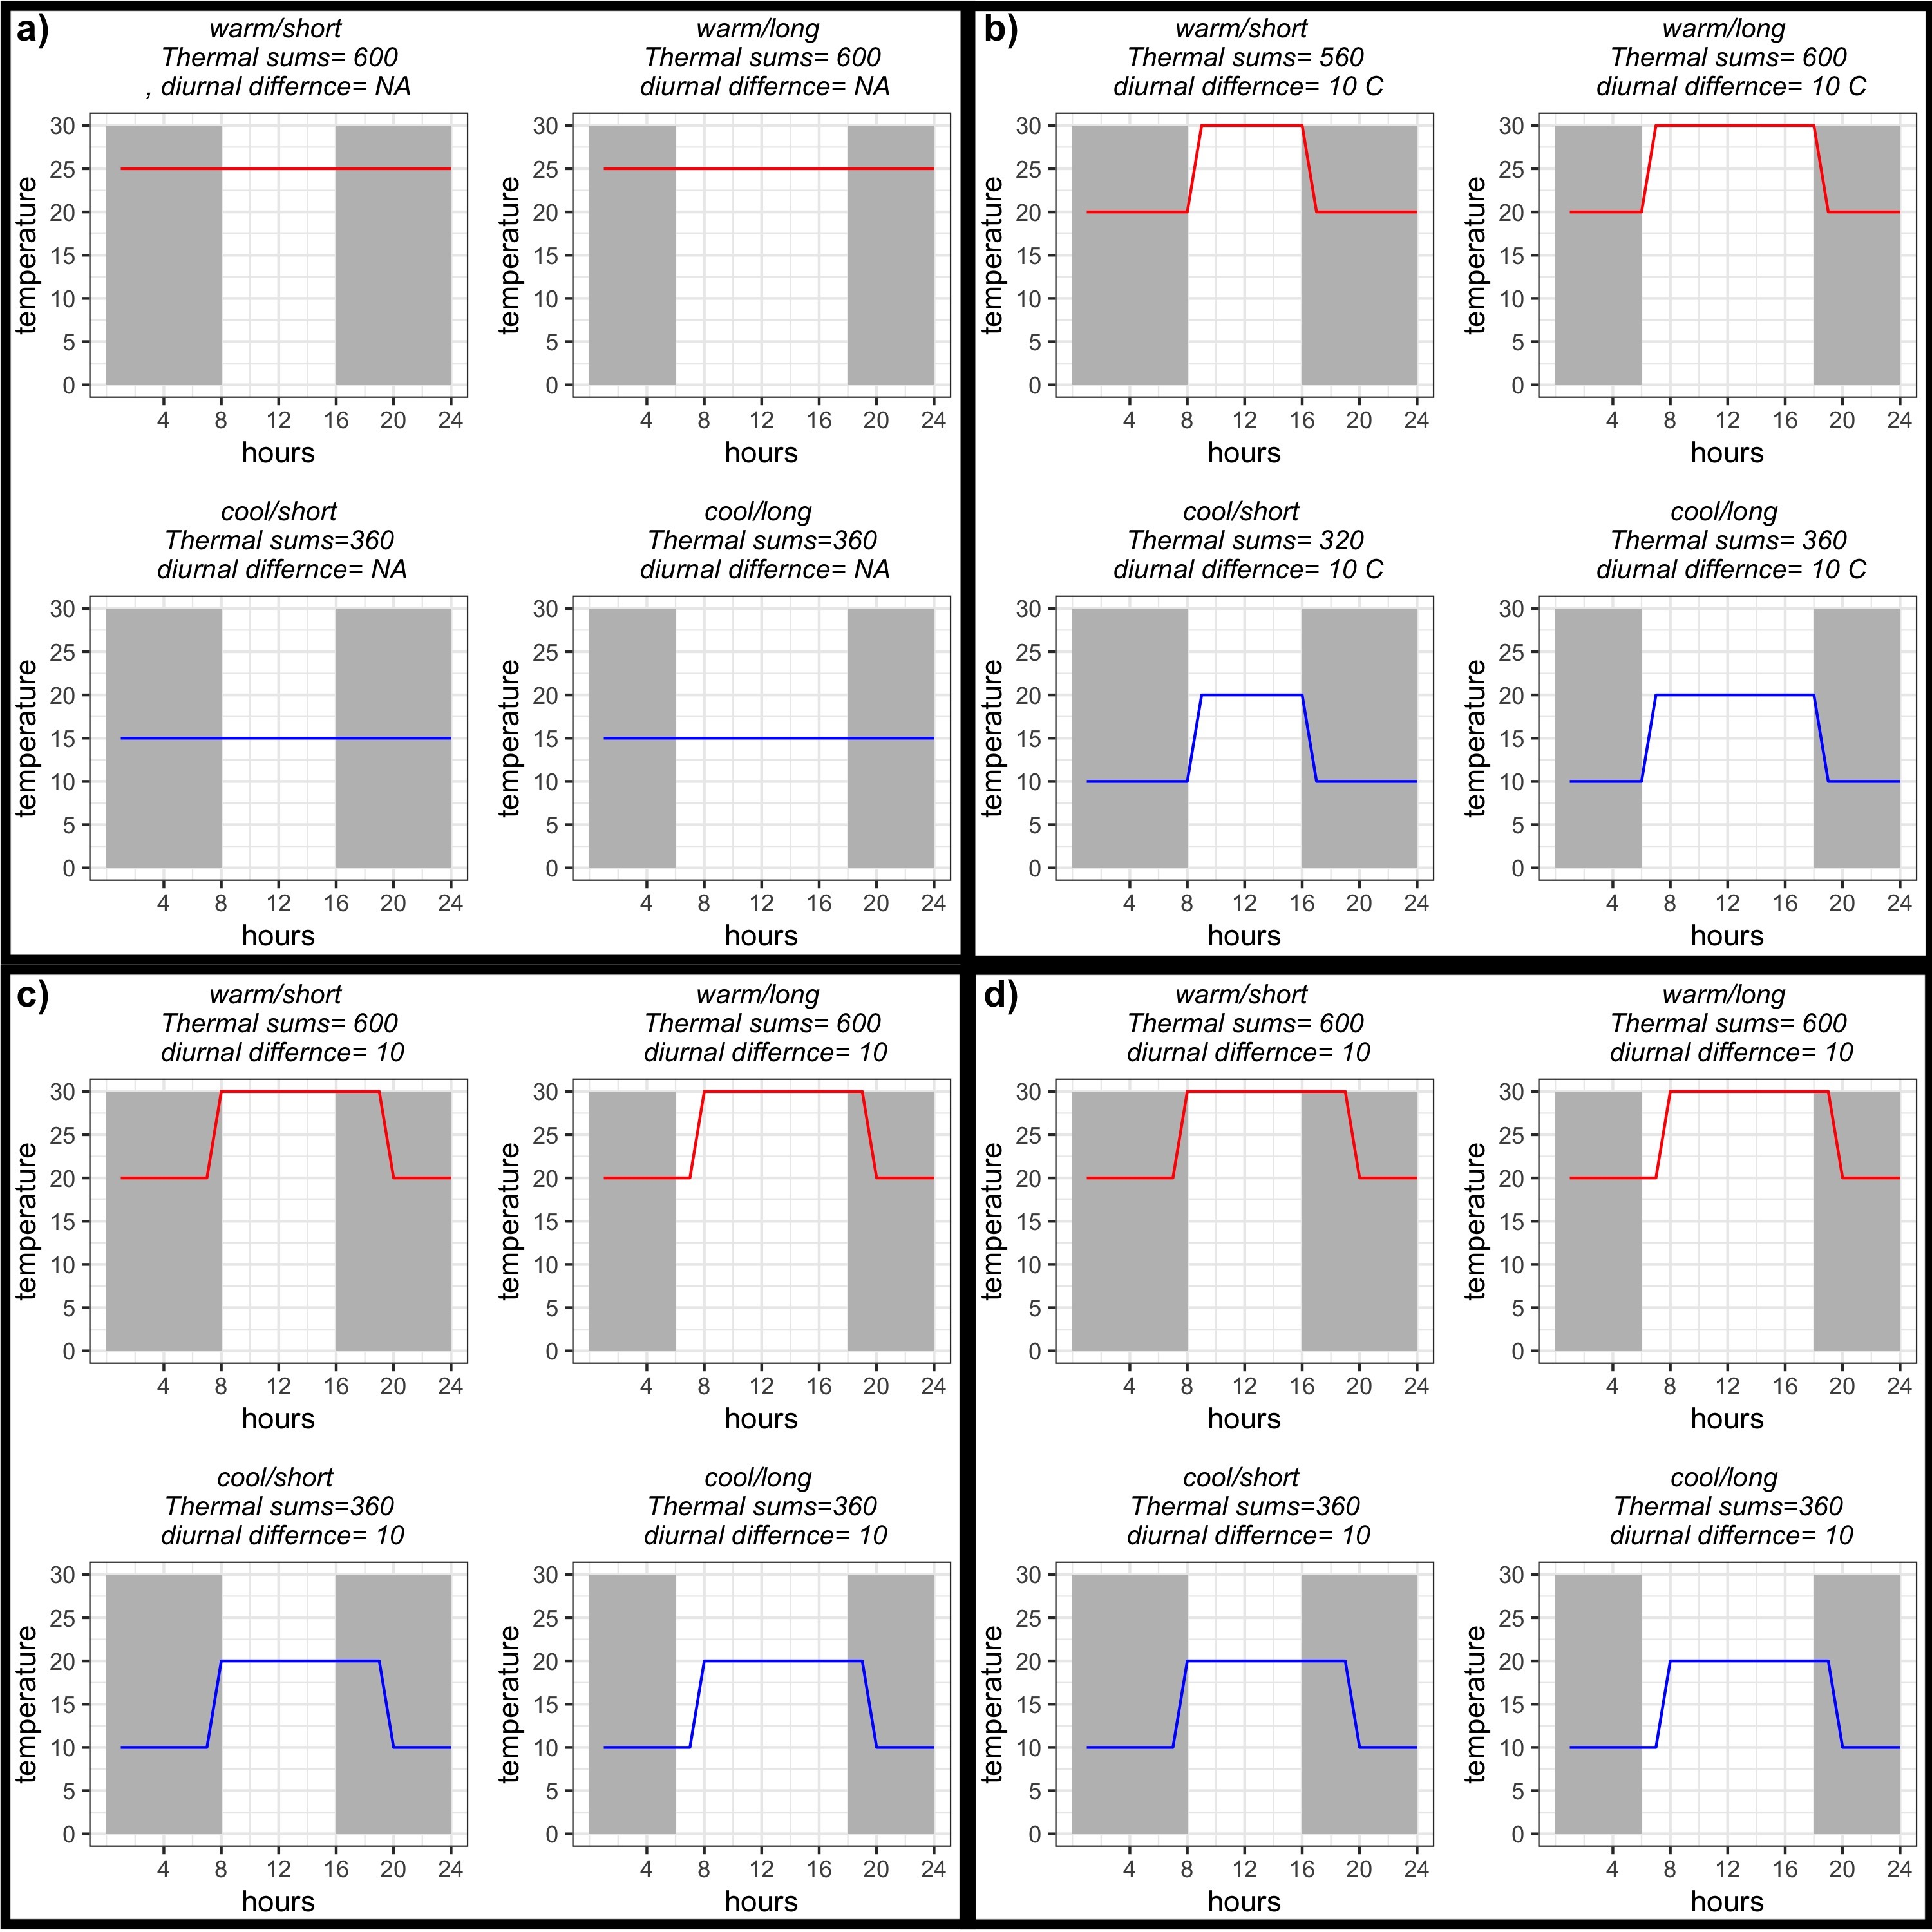
\includegraphics[width=\textwidth]{..//Plots/periodicity_figures/designs.jpeg}
    \caption{Conceptualized experimental designs to test temperature and daylength interactions on a biological response. In \textbf{a)} the design incorporates a standardize diurnal temperature fluctuation across all treatment. Because this thermoperiod is coupled with the photoperiod, while the same day and night temperatures are applied for the high and low temperature treatments respectively, the mean daily temperatures differ across each photoperiod treatment generating non-orthogonality. Designs \textbf{b)},\textbf{c)} and \textbf{d)} are all designs that can  correct this non-orthogonality. Design \textbf{b)}  manipulated temperature intensity only (no thermoperiodicity).% sacrificing some biological realism if the biological response in question requires diurnal temperature fluctuations. 
    In  \textbf{c)} photo- and thermo- periods are still are coupled but the orthogonality of mean daily temperature is maintained by proportionately varying the diurnal temperature fluctuations across treatments. %However, if temperature and light intensity interact biologically, this approach introduce unbalance and non-orthogonality introducing a new latent difference among the treatments in the form of diurnal temperature range.
    In design \textbf{d)} standard diurnal temperature fluctuations are maintained but, thermoperiod and photoperiod are decoupled and varied independently, maintaining orthogonality daily mean temperatures.}% but may introduce inferential bias as the periodicity of temperature relative to temperature will be non-orthogonal among treatment combination.} 
    \label{fig:ortho}
\end{figure}
 

\end{document}




\begin{enumerate}
\item Temperature and light control and signal many biological processes.
\item They often interact, substitute or compensate for each other.
\item A major goal of biology is to quantify their effects and interactions
\item This has become extra important for predicting organism's response to global change
\item This task cannot be done well through observational studies as light and temperature regimes usually co-vary
\item Experiments in controlled environments (growth chambers, greenhouses etc) can do this, using experimental treatment to partition the effects of this variables and their interactions.
\item Indeed much progress has been made with this approach
\item But experiments must balance many competing factors in their designs, biological realism with statistical inference, the effect of unmeasured climate variable, blocking effects etc.
\item In the sections below we highlight a particular problem that can arise when designing experiments to partition the effects of temperature and daylength and understand their interaction. Our example uses woody plant phenology as an example, but the approach we detail here is relevant for other organisms and biological process too.  
\end{enumerate}

\section{Phenological response to Temperature and Light}
Here a very brief (one paragraph) overview of how light and temperature influence spring phenology. Keep it basic (Warming accelerate phenology, photoperiod might be a threshold), acknowledge chilling is important too, but our example won't really focus on it. Leave some open questions about their interactive nature.

\section{Testing Interactions}
\begin{enumerate}
\item To test interactions and partition effects among two variables that co-vary in nature one must:
\item Have at least 2 treatment levels of each variable of interest
\item Apply them orthoganigally, factorially (\ref{fig:examp}, blue box) and define these terms.
\item This may seem obvious but is rarely done. In the case of phenology, a recent analysis of controlled enviroonment study found that only X of Y studies manipulated both light and temperature cues in the same experience and only Z of X did so orthoginally.
\end{enumerate}
\section{Axes of environmental variation annd their there problem}
\begin{enumerate}
\item A further complication arises when decided how to apply each treatment.
\item For any environmental variable there are two axes of variation that can be manipulated in an experiment.  
\item Intensity: Temperature, luminosity. 
\item Period: Thermoperid, Photoperiod.
\item There are measures that incorperate both period intensity (ie growing degree hours).
\item For light cues, photoperiod is the primary phenolgoical cure
\item For temperature, period and intesity matter. For example, temperture in nature varies diurnally and dirunal temperature fluctions may contribute to the phenology signal, or at the very least, lack of them might make phenology wonky. 
\item Therefore a common approach in experiments that seems to balance prior knowlege, biological realism and experimental inferences is to vary photo period, and temperature intensity and period. 
\item Clarify with an example. 12 and 8 hours of daylength. 30/20 and  20/10 temperature (or whatever I said in the figure).
\item If not carefully handled this approach can introduce a nonorthogicanity into the experiment, biasing inference.
\item If the thermo-periodicity and photoperiodcity are coupled (ie the night time temperatures begin when the lights go off, and the day time temperatures begin when they turn back on) The impact is that that the high temperautre high/long photoperod treatment more cumulative heat than the high temperature/short photoperiod treatment throughout the experiment as can be seem when the temperature treatment are converted to thermal sums (\ref{fig:examp},(\ref{fig:ortho}b)). To state this more simply, though the applied temperatures are the same sicne their are applied for different durations, the mean daily temperature differ among the temperature treatments.
\item This non-orthoginality makes it stasticially impossible to differentiate the effect of the photoperiod and temperature treatments.
\end{enumerate}
\section{Quantifying uncertainty}
\begin{enumerate}
\item To estimate the extent to which this non-orthangonical could bias results we intergated the results from a large scale experiment that included a coupled thermo-photoperid design. We used plane geometry to estimate how much of the estimated forcing effect (the assumed dominant cue) may actually be attributed to change in photoperiod. The calcualtions can be found in the suppliment.
\item While the original model estimates of the forcing and photoperiod effects (phenological sensitivy; $\Delta$ phenological event day/ $\Delta$ cue level) were estimate 9.5 and 4.5 advance we estimate that as much about 3.0 (units?) of the forcing effect could be attributed to the photoperiod effect.
\item It is important to stress that this is not a model correction. The original model could acutally before correct or it could in fact have understimated the true forcing effect and infalted the photoperiod effect. We simply cannot say this. (\textit{Probably should think about how to phase all this without making it seem like the Flynn paper is wrong}).
\item Our estimate of ``how much of the reported photo-period response could in actuality be driven by the latent differences in thermo-period" can be rephrased as a prediction of the expected difference in estimated photoperiod sensitivity between a coupled and decoupled photo- and thermo-period experiment.
\item While we are aware of no experiments that explicitly test these different designs, a phenological study by \citet{Buonaiuto:2021ug} applied serveral treatments levels that overlap with those in the \citet{Flynn2018} study to twig cuttings from the same source population. However in the second study the authors decoupled photo- and thermo-period. After subseting each dataset to  include nly species and treatment levels common amoung them, we re-analyzed the data (see supplimental method) and found that difference in the average response to photoperiod amoung study designs  was on the same order our mathmatical prediction see figure, though the photoperiod effect was in fact weaker in the uncoupled dataset (\ref{tab:compy}).\\
\item  With such significant uncertainty in partitioning the effect of forcing and photoperod even in experiment, this might contribute to the debate about the importance of photoperiod.
\item Below we outline several solutions to this experimental design, that should inprove the inference from growth chamber studies
\end{enumerate}

\section{Solutions}
\begin{enumerate}
\item Manipulate temperature intesity only and photoperiod. You estimate interactions because you have multiple levels of temperature and orthogiality. Lose some biological realism (\ref{fig:ortho}a).


\item Uncouple thermoperiod and photoperiod. As done in \citet{Buonaiuto:2021ug}. While this is probably better than coupled approach as it account for statistical interaction, it may introduce new artifact that occur from biological interactions. For example evidence from horticulture studies have demonstrated that cell growth is most sensitive to temperature fluctuation at the beginning of the photoperiod\citep{Erwin1998}. \citet{Erwin1998} found that increasing temperatures in the first two hours of the photoperiod was almost as effective for stimulating shoot elongation as similar temperature increases for the whole photoperiod (\ref{fig:ortho}c).

\item Set temperature treatments using metrics that account for period and intestist. Growing degree hours.maintain mean temperature and set photoperiod legnths and thus thermal orthoginality in expiriment by proportionately varying diurnal fluctionation accross treatment level. However, if the differenes between day and night temperature has a meanful biological effect as has been shown, this introduces another confonding, non-orthoginal factor (\ref{fig:ortho}d).

\item While this improvements should improve our ability to assess light and temperature interactions in biology, their challenges should aslo remind us to be humble with inference and think critically about what is, and isn't accounted for.
\end{enumerate}

%EMW20Feb22: I feel like the chilling details are not critical ... see what you think of above edits 
% CUT: are usually applied in a pre-treatment either by sequentially removing plant materials from the field throughout the winter dormancy period \citep{limitingcues} or applying experimental chilling in a cold chamber before warm temperature and light treatments are applied in tandem \citep{Weinberger:1950aa,Flynn2018
